\documentclass[aspectratio=169]{beamer}
%\usetheme{Boadilla}
%\usetheme{default}
%\usecolortheme[snowy]{owl}
\usecolortheme{owl}
\usepackage{color}
\usepackage{fontawesome}
\usepackage{tikz}
\usetikzlibrary{arrows,calc,positioning}
\usepackage{hyperref}
\hypersetup{
    colorlinks=true,
    linkcolor=blue,
    filecolor=magenta,      
    urlcolor=blue,
}

\urlstyle{same}



\newcommand{\exurl}[1]{\texttt{www.shop.xyz/#1}}
\newcommand{\attacker}{the attacker}
\newcommand{\Attacker}{The attacker}
\newcommand{\eve}{Eve\ }
\newcommand{\alice}{Alice\ }

\title{\textbf{You've Been Hacked}}
\subtitle{An (Interactive) Course on Web Security\newline\vfill}
\author{\textbf{Paul Duplys}}
\institute[]{\faTwitter\hspace{0.1cm} @duplys \hspace{1cm} \faGithub\hspace{0.1cm} duplys \hspace{1cm} \faLinkedinSquare\hspace{0.1cm} linkedin.com/in/paulduplys/}
\date{}

\begin{document}

{
\usebackgroundtemplate{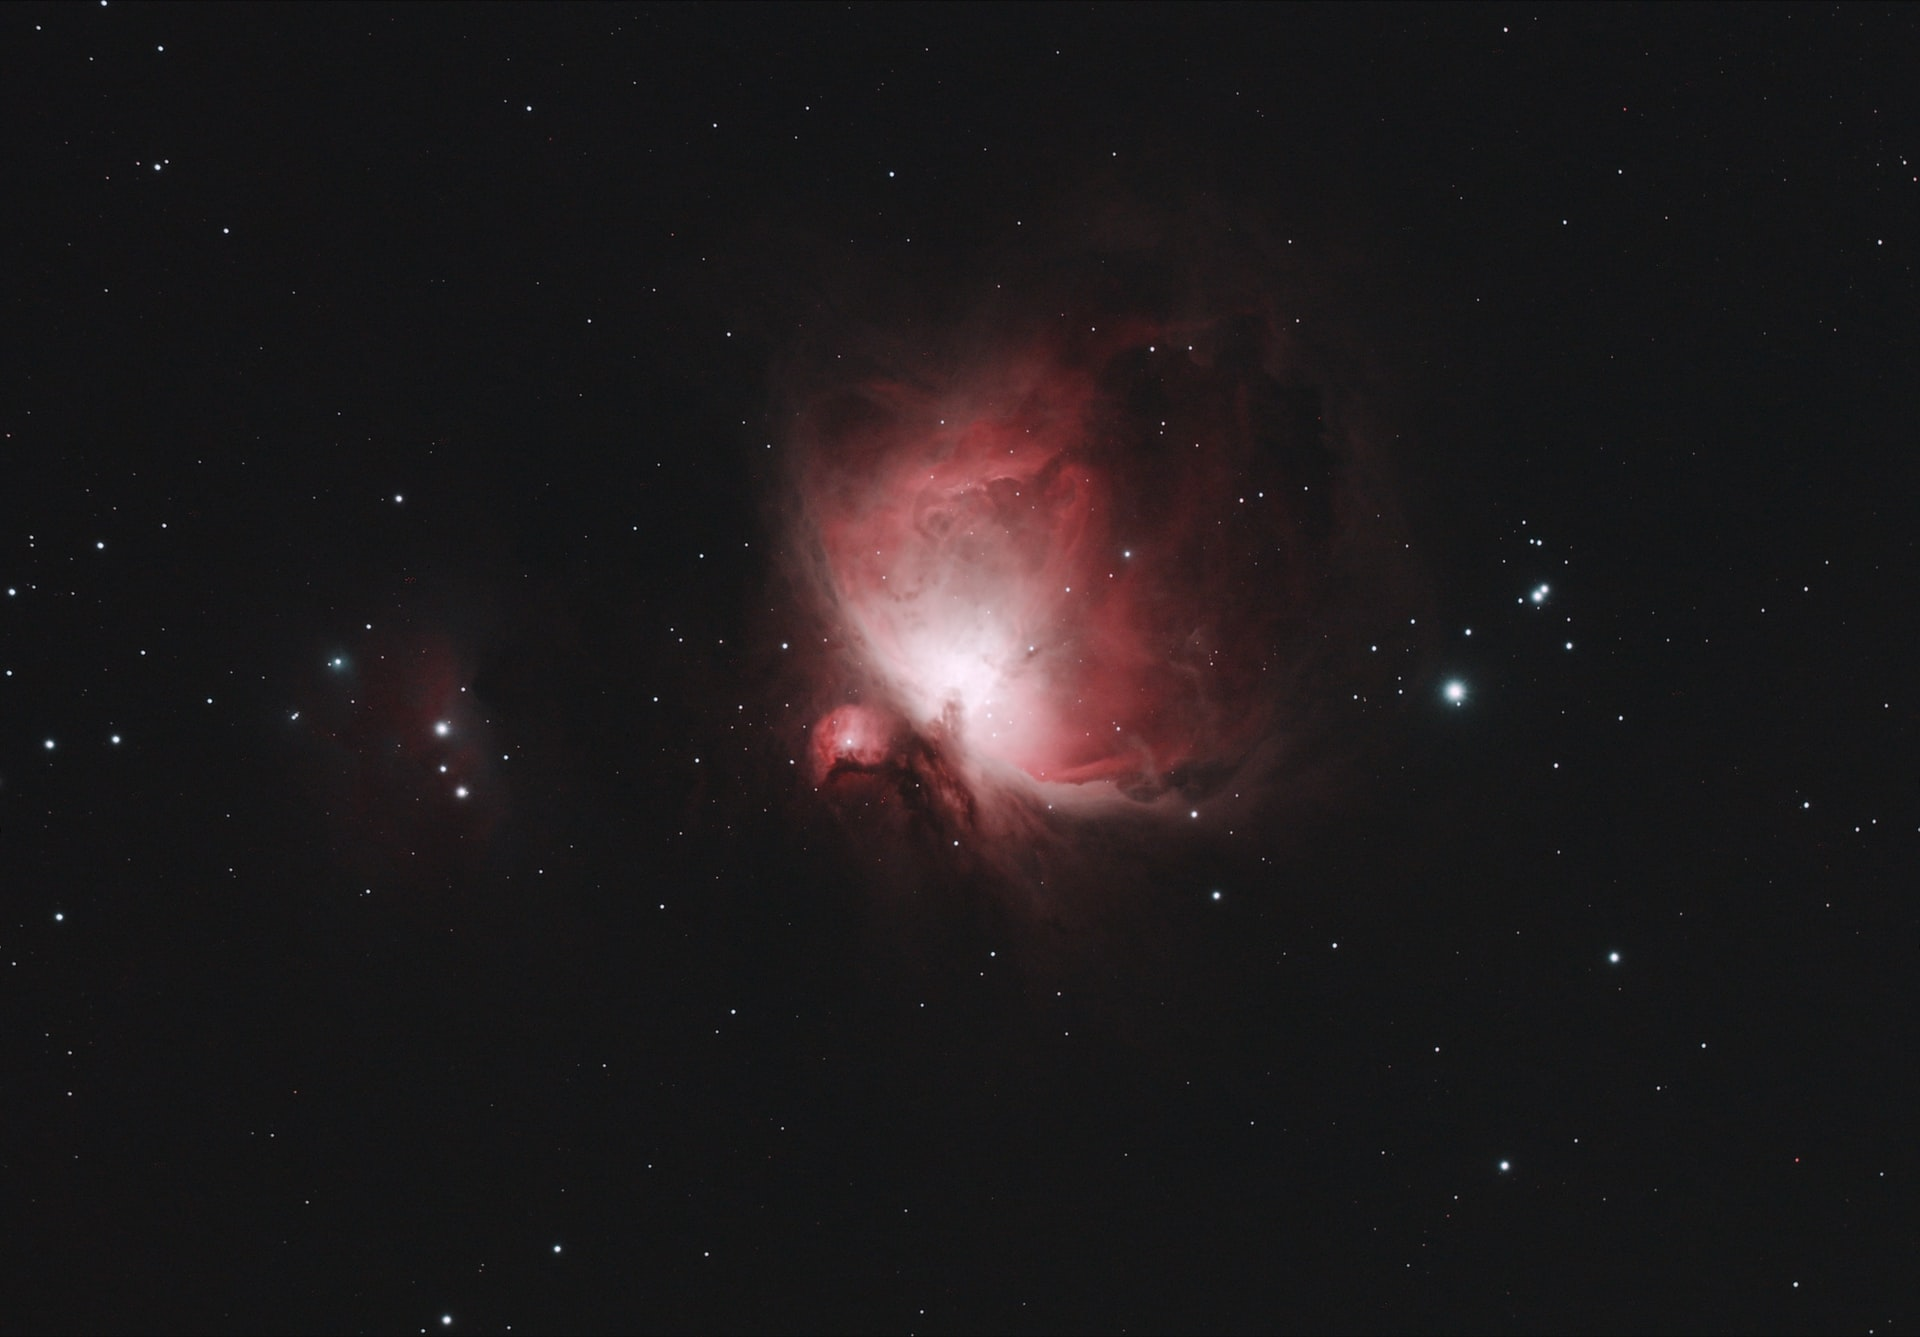
\includegraphics[width=\paperwidth]{./img/orion-nebula.jpg}}
\begin{frame}
    \titlepage
\end{frame}
}

\begin{frame}
    %\frametitle{Outline}
    \tableofcontents
\end{frame}

\begin{frame}
    \frametitle{\texttt{man slides}}

    (Interactive) course on web security based on Carsten Eiler's book "You've Been Hacked".
    
    Who is the audience? How can I use the book? How can I explore the app?
\end{frame}

\begin{frame}
    \frametitle{\texttt{whoami}}
    short intro/bio.
\end{frame}

%%%%%%%%%%%%%%%%%%%%%%%%%%%%%%%%%%%%%%%%%%%%%%%%%%%%%%%%%%%%%%%%%%%%%%%%%%%%%%%
%%% 0x0: Preliminaries %%%%%%%%%%%%%%%%%%%%%%%%%%%%%%%%%%%%%%%%%%%%%%%%%%%%%%%%
%%%%%%%%%%%%%%%%%%%%%%%%%%%%%%%%%%%%%%%%%%%%%%%%%%%%%%%%%%%%%%%%%%%%%%%%%%%%%%%

\section{0x0: Preliminaries}

{
%\usebackgroundtemplate{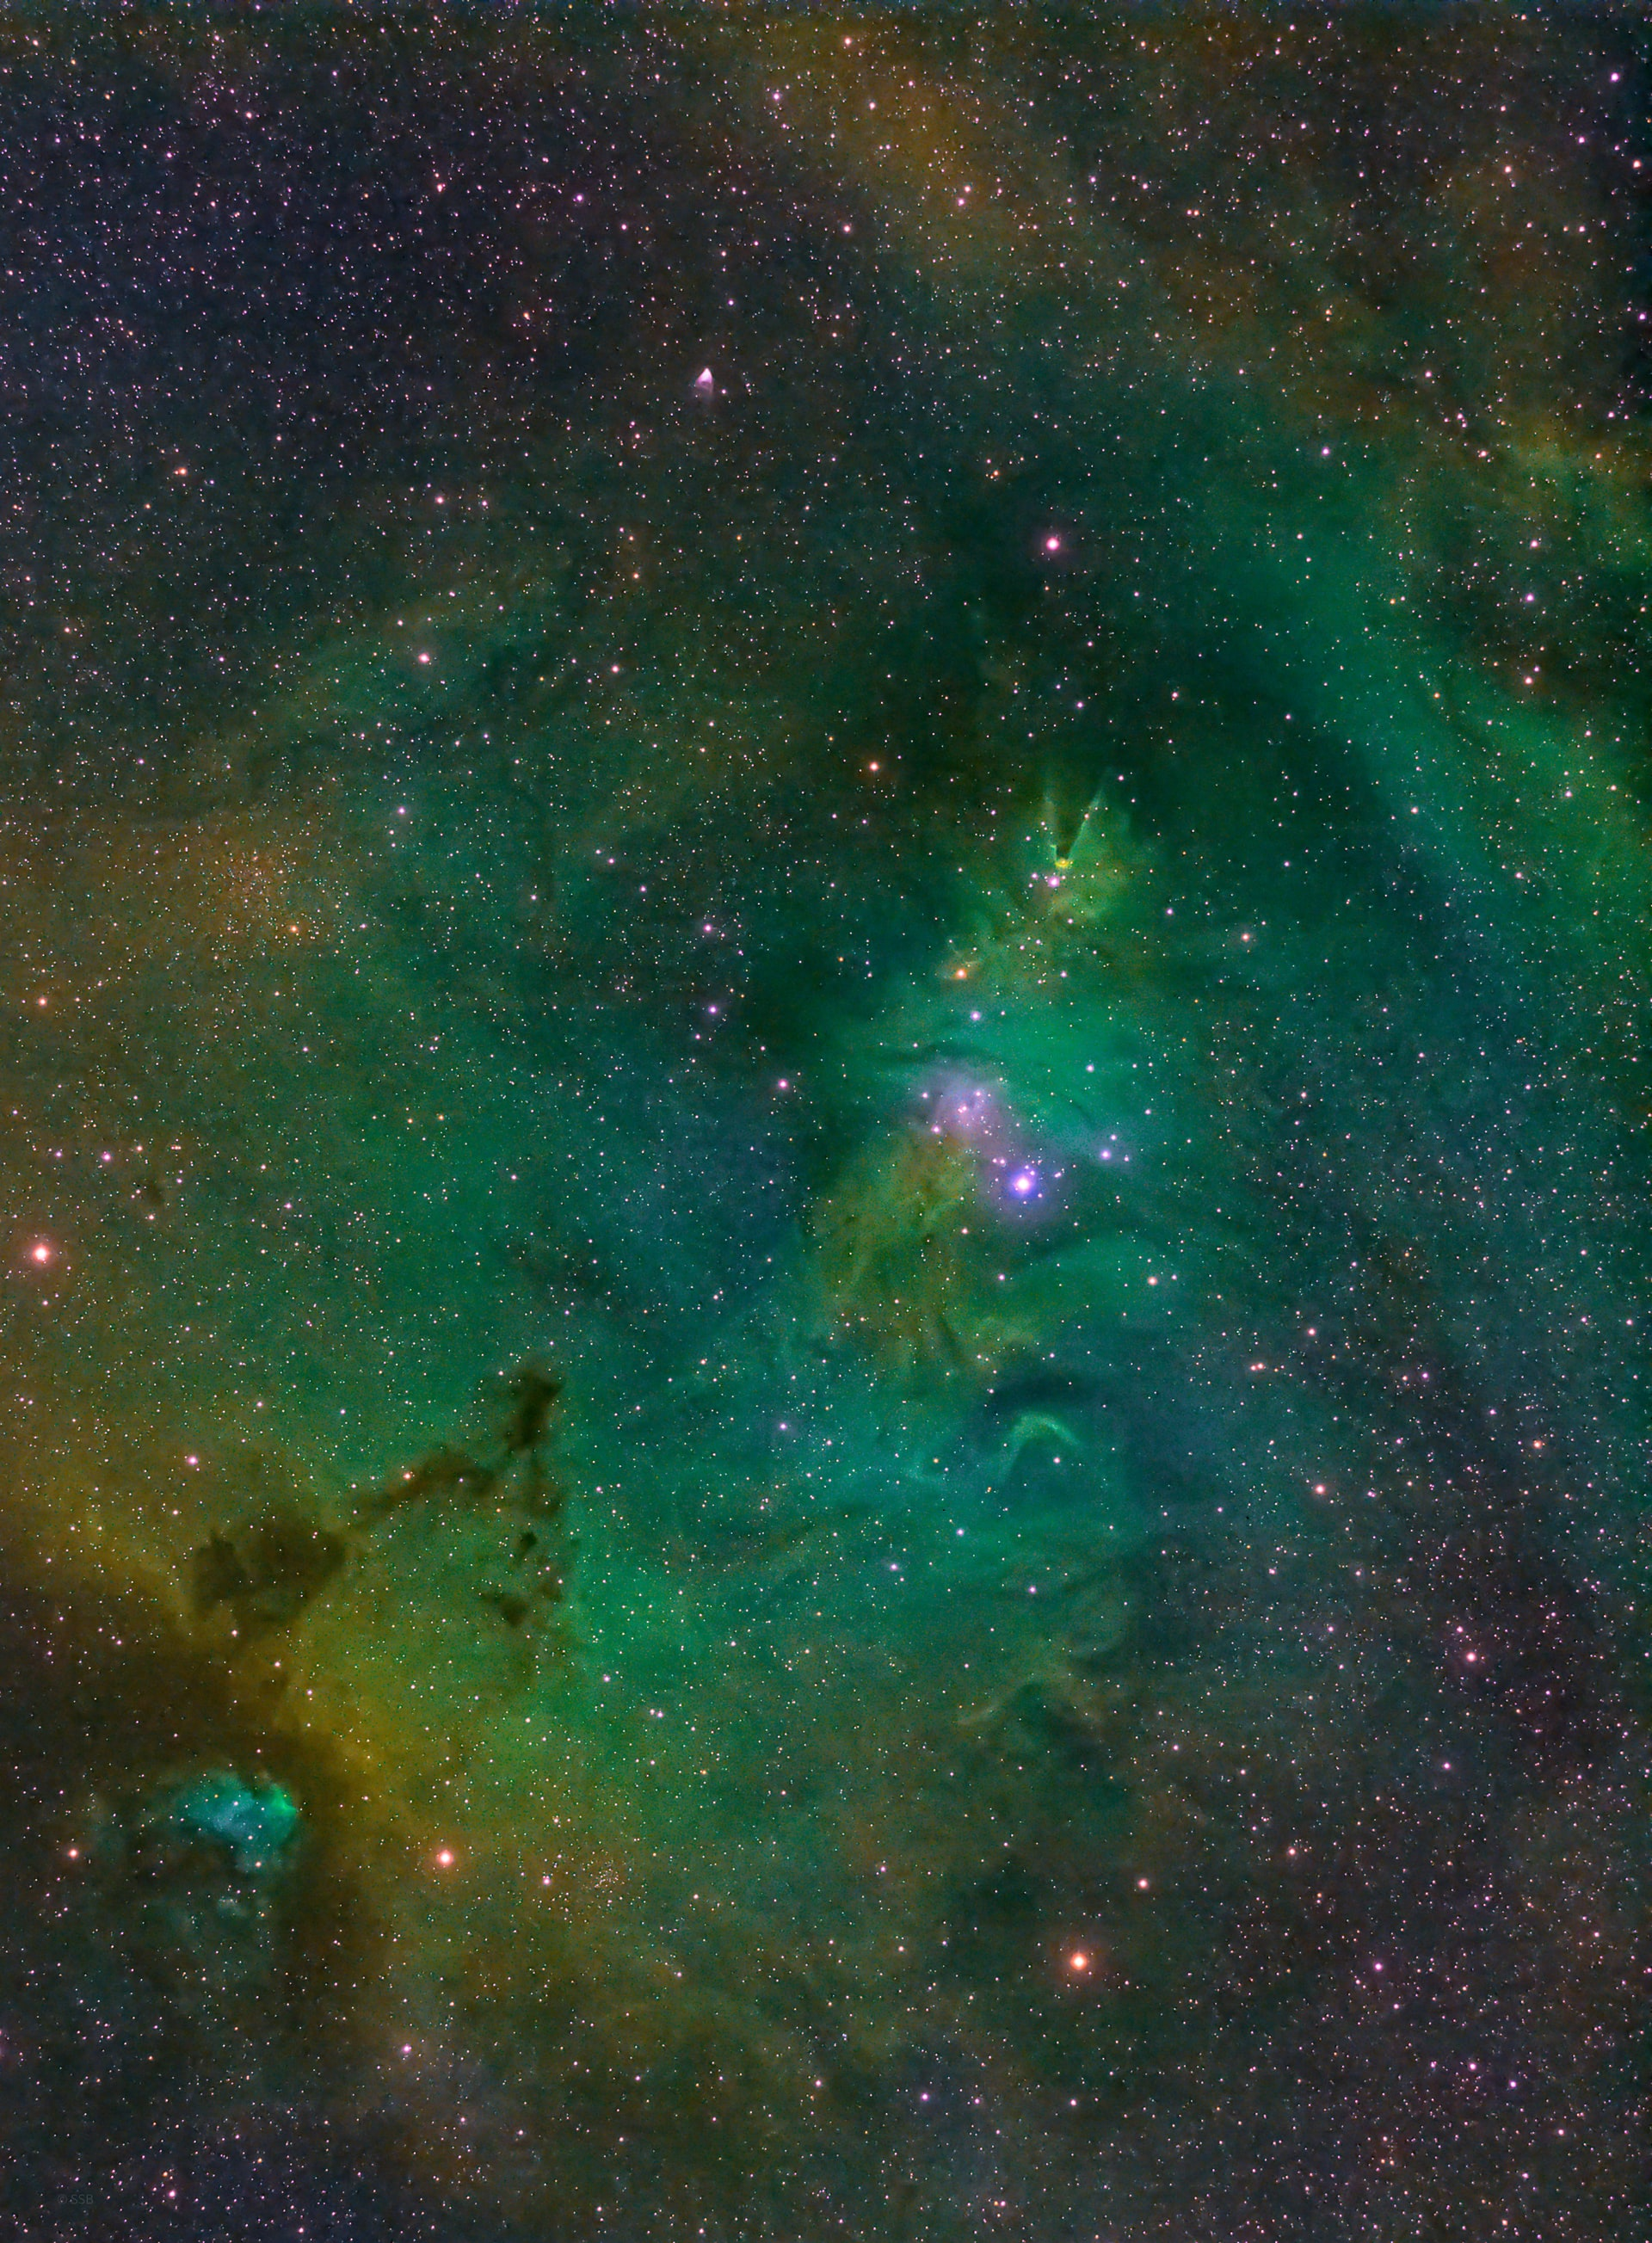
\includegraphics[width=\paperwidth]{./img/aldebaran.jpg}}
\begin{frame}
\huge{\textcolor{white}{\textbf{0x0: Preliminaries}}}
\end{frame}
}

\begin{frame}
	\frametitle{Conventions}
	\begin{itemize}
		\item Alice, Bob: legitimate users
		\item Eve: malicious user, attacker
		\item Server: web server running a web application
		\item Client: web browser (or computer running the web browser)
	\end{itemize}
\end{frame}

\begin{frame}
	\frametitle{GitHub Repo}
	\begin{itemize}
		\item \url{https://github.com/duplys/youve-been-hacked}
		\item Dockerfile \& setup instructions
		\item Write-ups
		\item Code
	\end{itemize}
\end{frame}

\begin{frame}
	\frametitle{Build Docker Image}
	\begin{itemize}
		\item Running the demo web application in a Docker container is the easiest way to get started
		\item \texttt{Docker} dir contains \texttt{Dockerfile} for the vulnerable web application
		\item \texttt{Makefile} (\texttt{make build}) or \texttt{docker-compose}
	\end{itemize}
	
\end{frame}

\begin{frame}[fragile]
	\frametitle{Starting Docker Containers}
	\begin{itemize}
        \item You'll need an empty directory \texttt{tmp} in the \texttt{Docker} dir
		\item In \texttt{Docker} dir, run \verb|$ docker-compose up|
	\end{itemize}
\end{frame}

\begin{frame}[fragile]
	\frametitle{Accessing ZAProxy}
	\begin{itemize}
		\item In your web browser, hit \verb|http://127.0.0.1:8080/zap/|
        \item For documentation, see \url{https://www.zaproxy.org/docs/docker/webswing/}
	\end{itemize}
\end{frame}

\begin{frame}[fragile]
	\frametitle{Accesing the vulnerable Web application}
	\begin{itemize}
		\item \verb|$ docker container inspect docker_vulnapp_1 | grep "IPAddress"|
	\end{itemize}
\end{frame}

\begin{frame}[fragile]
	\frametitle{Cleaning Up}
	\begin{itemize}
		\item Run \verb|$ docker-compose down|
	\end{itemize}
\end{frame}


% Next, go your web browser and visit `http://127.0.0.1:8080/zap/` (as [described here](https://www.zaproxy.org/docs/docker/webswing/))

Next, you'll need the IP address of the Docker container running the vulnerable application. To extract this, do:

```shell
$ % docker container inspect exciting_maxwell
[
	{
		"Id": "9ea057ec1cea78eb1ab3abe4ba9f1cadb42ab751bf7bc1c9b0f277a286eeeddf",
		"Created": "2020-11-20T19:35:08.9811261Z",
		
		-- snip --
		
		"Networks": {
			"hack-network": {
				"IPAMConfig": null,
				"Links": null,
				"Aliases": [
					"9ea057ec1cea"
				],
				"NetworkID": "84aadd9f11e09968530e5093bdb8c95df7f30aa7efa7526ab315e30558126e03",
				"EndpointID": "adc8e373fe433540b208498a592d3598d79cb46ab860d1a302301ae9378136b2",
				"Gateway": "172.19.0.1",
				"IPAddress": "172.19.0.2",
				"IPPrefixLen": 16,
				"IPv6Gateway": "",
				
				-- snip --
				```
				
				You'll need to import the dynamic SSL certificate into Firefox. (go to ZAP --> Option -> Dynamic SSL Certificates and download one...). 
				
				Now, in your Firefox browser you need to enter the following URL: `http://host.docker.internal:8888/daten/kapitel1.html`. The reason for this is that if you use `127.0.0.1` together with the ZAP proxy, once that HTTP request arrives at the proxy, the proxy running in a docker container tries to resolve it and hits itself. So you get a "connection refused" warning and a Bad Gateway HTML response.


\begin{frame}
    \frametitle{Fahrplan}

    \begin{itemize}

    \end{itemize}

\end{frame}

%%%%%%%%%%%%%%%%%%%%%%%%%%%%%%%%%%%%%%%%%%%%%%%%%%%%%%%%%%%%%%%%%%%%%%%%%%%%%%%
%%% 0x1: Recon %%%%%%%%%%%%%%%%%%%%%%%%%%%%%%%%%%%%%%%%%%%%%%%%%%%%%%%%%%%%%%%%
%%%%%%%%%%%%%%%%%%%%%%%%%%%%%%%%%%%%%%%%%%%%%%%%%%%%%%%%%%%%%%%%%%%%%%%%%%%%%%%



\end{document}